% !TEX program = xelatex
% BeforeTap - native Android and iOS product design specification
% Prepared for Suthankan Balenthiran, 20 November 2026.
\documentclass[10pt,a4paper]{article}
\usepackage{fontspec}
\usepackage[margin=19mm,headheight=22pt,headsep=8mm,footskip=12mm]{geometry}
\usepackage{xcolor,graphicx,booktabs,tabularx,longtable,array,multicol,amssymb}
\usepackage{enumitem,titlesec,fancyhdr,hyperref,tcolorbox,tikz,lastpage}
\usepackage{xurl}
\usetikzlibrary{arrows.meta,positioning,shapes.geometric}
\defaultfontfeatures{Ligatures=TeX}
\setmainfont{Nimbus Sans}
\setsansfont{Nimbus Sans}
\definecolor{ink}{HTML}{142037}
\definecolor{deep}{HTML}{0B1424}
\definecolor{muted}{HTML}{596B80}
\definecolor{teal}{HTML}{008F82}
\definecolor{mint}{HTML}{DDF7F1}
\definecolor{bluegray}{HTML}{F1F5F9}
\definecolor{line}{HTML}{DCE5EB}
\definecolor{amber}{HTML}{B96D12}
\definecolor{softamber}{HTML}{FFF2DC}
\definecolor{coral}{HTML}{C64248}
\definecolor{softcoral}{HTML}{FFF0F0}
\definecolor{success}{HTML}{157C59}
\definecolor{softsuccess}{HTML}{E8F8EE}
\hypersetup{colorlinks=true,linkcolor=teal,urlcolor=teal,pdftitle={BeforeTap - Product and Native UI/UX Design Specification},pdfauthor={Prepared for Suthankan Balenthiran},pdfsubject={Android and iOS native mobile app design}}
\pagestyle{fancy}
\fancyhf{}
\fancyhead[L]{\textcolor{teal}{\bfseries BEFORETAP} \textcolor{muted}{/ PRODUCT DESIGN}}
\fancyhead[R]{\textcolor{muted}{v1.0  |  20 NOV 2026}}
\fancyfoot[L]{\textcolor{muted}{Confidential working specification  /  Suthankan Balenthiran}}
\fancyfoot[R]{\textcolor{muted}{\thepage\ / \pageref{LastPage}}}
\renewcommand{\headrulewidth}{0.4pt}
\renewcommand{\headrule}{\hbox to\headwidth{\color{line}\leaders\hrule height \headrulewidth\hfill}}
\titleformat{\section}{\color{ink}\sffamily\bfseries\Large}{\thesection}{0.75em}{}[\vspace{-3pt}\color{teal}\titlerule]
\titleformat{\subsection}{\color{ink}\sffamily\bfseries\large}{\thesubsection}{0.6em}{}
\titleformat{\subsubsection}{\color{ink}\sffamily\bfseries\normalsize}{\thesubsubsection}{0.6em}{}
\titlespacing*{\section}{0pt}{16pt}{9pt}
\titlespacing*{\subsection}{0pt}{12pt}{6pt}
\setlength{\parindent}{0pt}
\setlength{\parskip}{5pt}
\renewcommand{\arraystretch}{1.2}
\setlist[itemize]{leftmargin=*,topsep=3pt,itemsep=2pt}
\setlist[enumerate]{leftmargin=*,topsep=3pt,itemsep=2pt}
\newcolumntype{Y}{>{\raggedright\arraybackslash}X}
\newtcolorbox{featurebox}[1][]{colback=bluegray,colframe=line,boxrule=.5pt,arc=2.5mm,left=4mm,right=4mm,top=3mm,bottom=3mm,#1}
\newtcolorbox{greenbox}[1][]{colback=mint,colframe=teal,boxrule=.7pt,arc=2.5mm,left=4mm,right=4mm,top=3mm,bottom=3mm,#1}
\newtcolorbox{riskbox}[1][]{colback=softamber,colframe=amber,boxrule=.7pt,arc=2.5mm,left=4mm,right=4mm,top=3mm,bottom=3mm,#1}
\newcommand{\pill}[2]{\tcbox[on line,boxrule=0pt,arc=1.6mm,colback=#1,left=2mm,right=2mm,top=1mm,bottom=1mm]{\footnotesize\bfseries #2}}
\newcommand{\spec}[2]{\textbf{#1}\quad #2\par}
\newcommand{\platform}[1]{\vspace{1mm}\textcolor{teal}{\bfseries #1}\par}
\newcommand{\UIRow}[4]{\textbf{#1} & #2 & #3 & #4 \\ \midrule}
\begin{document}

\begin{titlepage}
\pagecolor{deep}\color{white}
\vspace*{21mm}
{\color{white}\Huge\bfseries BeforeTap\par}
\vspace{3mm}
{\color{mint}\LARGE Pause. Check. Act.\par}
\vspace{18mm}
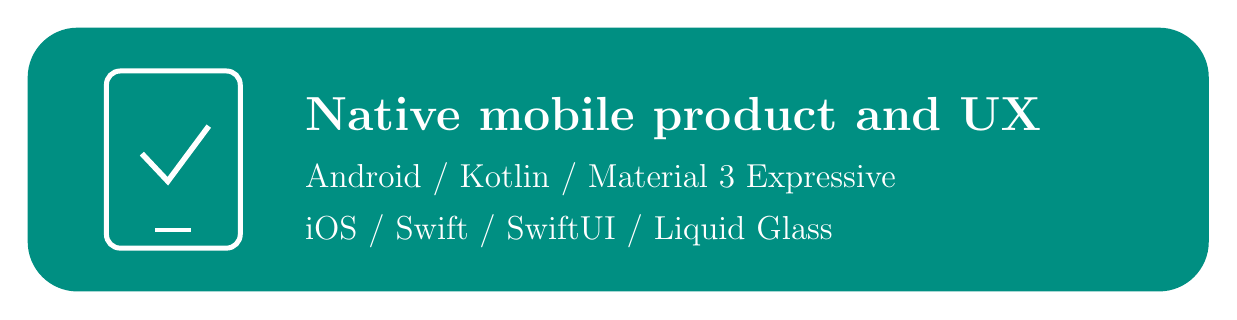
\begin{tikzpicture}
  \fill[teal,rounded corners=18pt] (0,0) rectangle (15,3.35);
  \draw[white,line width=1.8pt,rounded corners=5pt] (1.0,.55) rectangle (2.7,2.8);
  \draw[white,line width=1.2pt] (1.62,.78)--(2.08,.78);
  \draw[white,line width=2pt] (1.45,1.75)--(1.78,1.40)--(2.30,2.10);
  \node[anchor=west,text=white,font=\bfseries\LARGE] at (3.4,2.2) {Native mobile product and UX};
  \node[anchor=west,text=white,font=\large] at (3.4,1.42) {Android / Kotlin / Material 3 Expressive};
  \node[anchor=west,text=white,font=\large] at (3.4,.77) {iOS / Swift / SwiftUI / Liquid Glass};
\end{tikzpicture}\par
\vspace{18mm}
{\LARGE\bfseries Product, security and native UX\par}
\vspace{2mm}
{\LARGE\bfseries specification\par}
\vspace{5mm}
{\large Version 1.0  /  20 November 2026\par}
\vspace{18mm}
\begin{tabular}{@{}ll@{}}
\textcolor{mint}{Prepared for} & \textbf{Suthankan Balenthiran} \\
\textcolor{mint}{Project} & Two separate editable Figma Design files \\
\textcolor{mint}{Audience} & Product, UX, Android, iOS, security and QA \\
\textcolor{mint}{Status} & Design proposal, not a deployed security service \\
\end{tabular}
\vfill
{\color{mint}\small Concept design. Threat scores, verification and data handling require implementation, evaluation, and legal/platform-policy review before release.\par}
\end{titlepage}
\nopagecolor\color{ink}
\tableofcontents
\newpage

\section{Executive decision}
\begin{greenbox}
\textbf{Product promise.} BeforeTap helps a person pause before acting on a suspicious message, link, screenshot or QR code. In a few seconds, it surfaces concrete warning signs, makes uncertainty explicit, and offers one safe next step. It is a \emph{decision-support tool}, not an authority that certifies content as safe.
\end{greenbox}
\begin{tabularx}{\linewidth}{@{}p{31mm}Y@{}}\toprule
\textbf{Attribute} & \textbf{Design decision} \\ \midrule
Who & Mobile-first adults who regularly encounter unsolicited offers, payment instructions, delivery messages, job opportunities and suspicious links. Begin validation in Sri Lanka; retain international portability. \\
Job to be done & ``When an unexpected message asks me to act, help me understand the risk before I click, pay or share information.'' \\
Differentiator & Explainability + privacy by default + platform-native speed + practical independent verification guidance. \\
Primary entry & System share sheet; text/URL paste; screenshot/photo import; camera QR scan. \\
Primary outcome & A clear, evidence-led assessment and a safe action with no accidental opening of unsafe content. \\
Platforms & Separate Android and iOS implementations and separate Figma prototypes. Shared product semantics, distinct native components. \\
\bottomrule\end{tabularx}

\subsection{Design principles}
\begin{enumerate}
\item \textbf{Explain evidence, not magic scores.} Never present fabricated probability or imply an absence of detections guarantees safety.
\item \textbf{One decisive action.} Make ``Check something'' the clearest affordance on the home screen.
\item \textbf{Privacy precedes intelligence.} Process screenshots on-device; disclose URL lookups and minimize sensitive data.
\item \textbf{Clarity under stress.} Plain language, empathetic tone, no alarmist animations and no blame.
\item \textbf{Native feels native.} Preserve Apple and Android navigation, controls, typography, motion and accessibility behavior.
\item \textbf{Reduce irreversible mistakes.} Never auto-open suspicious URLs or start payments from a scan result.
\end{enumerate}

\section{Scope, assumptions and constraints}
\subsection{Now / next / later}
\begin{tabularx}{\linewidth}{@{}p{21mm}Y@{}}\toprule
\textbf{Release} & \textbf{Capabilities} \\ \midrule
MVP & Text and URL paste, image upload, on-device OCR, URL parsing, simple security rules, user-consented threat lookup, explainable results, independent-verification suggestions, optional local history, accessibility and basic privacy settings. \\
Next & Share extension/intent polish, safe QR decoding, URL expansion via protected server, domain registry signals, history search/filter, tailored reporting guidance, fully tested dark theme. \\
Later & On-device scam classification trained and evaluated on appropriate datasets; reliable Sinhala/Tamil processing after script support validation; family education; organization allowlists; verified reporting integrations where agreements exist. \\
\bottomrule\end{tabularx}

\subsection{Explicit non-goals}
\begin{itemize}
\item Automatically reading private WhatsApp conversations or all iOS messages.
\item Guaranteeing a link, sender, payment account, organization or job offer is legitimate.
\item Providing financial advice, recovering stolen funds, intercepting OTPs, or initiating transactions.
\item Selling messages/screenshots, aggressive advertising, or tracking behavior across apps.
\item A universal AI fraud model in v1; all model claims require holdout testing and calibrated evaluation.
\end{itemize}

\subsection{Core acceptance bar}
A person can share or paste a suspicious item, understand which checks ran, receive a result in four honest states, read two or more grounded reasons when available, and leave with a safe next step. A failed network call must never silently become a reassuring result.

\section{Research and user framing}
\subsection{Opportunity signals}
Sri Lanka CERT reported more than 12,650 complaints associated with online incidents and social-media misuse in 2025; this figure is not a count of scams alone [1]. Sri Lanka Police separately warns about online financial fraud through messaging services, fake opportunities and QR-code misuse [2]. The OECD identifies phishing, impersonation and fraudulent payment/investment requests as major consumer financial-scam risks [3]. These are \emph{problem signals}, not proof of product-market fit. Conduct local interviews and usability tests.

\subsection{Working personas}
\begin{tabularx}{\linewidth}{@{}p{29mm}Y Y@{}}\toprule
\textbf{Persona} & \textbf{Context / anxiety} & \textbf{Design response} \\ \midrule
Nila, 22 & University student, frequent job offers and shopping links; time-sensitive, fluent with native gestures. & Share-sheet entry, minimal taps, detailed domain evidence on demand. \\
Ravi, 42 & Works full time; gets delivery, banking and employment messages; cannot investigate deeply. & Direct risk summary, larger actions, clear independent-verification instruction. \\
Meena, 61 & Less confident with online scams, prefers understandable labels and a family member's guidance. & Accessible typography, nontechnical wording, visual + text risk cues, simple help flow. \\
\bottomrule\end{tabularx}

\subsection{Research tasks before build}
Interview at least 10 people across age and device types; ask them to show redacted examples, not personal messages. Test whether they recognize genuine domains, whether ``no known threat'' is misread as ``safe'', and what action they would take after each result. Translate findings into a revision log. Recruitment should not imply victims were careless.

\section{Information architecture and navigation}
\begin{figure}[h!]
\centering
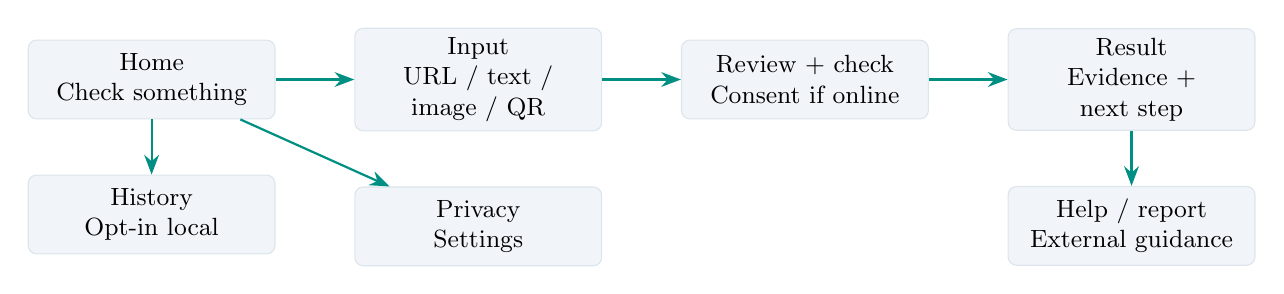
\begin{tikzpicture}[node distance=7mm and 10mm, every node/.style={font=\small},box/.style={draw=line,rounded corners=3pt,fill=bluegray,align=center,text width=29mm,minimum height=10mm},arr/.style={-{Stealth[length=2.5mm]},draw=teal,thick}]
\node[box] (home) {Home\\Check something};
\node[box, right=of home] (input) {Input\\URL / text / image / QR};
\node[box, right=of input] (analysis) {Review + check\\Consent if online};
\node[box, right=of analysis] (result) {Result\\Evidence + next step};
\draw[arr] (home)--(input);\draw[arr](input)--(analysis);\draw[arr](analysis)--(result);
\node[box,below=of home] (history) {History\\Opt-in local};
\node[box,below=of input] (privacy) {Privacy\\Settings};
\node[box,below=of result] (help) {Help / report\\External guidance};
\draw[arr] (home)--(history);\draw[arr] (home)--(privacy);\draw[arr] (result)--(help);
\end{tikzpicture}
\caption{The core journey is linear; secondary destinations do not obstruct the first scan.}
\end{figure}

\subsection{Navigation models}
\platform{iOS}
Three native tabs: \textbf{Check}, \textbf{History}, \textbf{Settings}. Use a standard SwiftUI tab bar in Liquid Glass; modal sheets for importing, confirmation and detailed evidence; NavigationStack for drill-down. The check button is a prominent in-content primary action rather than an Android-style FAB.
\platform{Android}
Three Material 3 navigation destinations: \textbf{Check}, \textbf{History}, \textbf{Settings}. Use adaptive navigation bar/rail as size requires; a prominent contained action or expressive FAB for Scan; modal bottom sheets for source selection; native predictive back behavior.

\section{End-to-end journeys}
\subsection{J1. Link via share sheet}
\begin{enumerate}
\item User chooses Share $\rightarrow$ BeforeTap from a supported app; the native import surface receives the link.
\item Preview displays the full hostname in readable type. Remove tracking/query secrets from analytics and logs.
\item User taps \emph{Check link}; app runs local URL parsing, impersonation checks and, after consent where appropriate, threat lookup.
\item Result states what was checked and which sources were available. Unknown is never displayed as safe.
\item User may expand evidence or choose \emph{How to verify independently}; external opening is never automatic.
\end{enumerate}
\subsection{J2. Suspicious screenshot}
\begin{enumerate}
\item User imports a screenshot from Photos/Gallery or the system share action.
\item Local OCR extracts text; the user sees/edit-corrects the extracted text before checking.
\item App highlights relevant sentences (urgency, requests for credentials, fees, unfamiliar links).
\item It presents understandable reasons, suggested next action, and optional local history.
\end{enumerate}
\subsection{J3. QR code}
Camera permission is requested at scan time, not during onboarding. The scanner extracts bytes without following URLs. The user previews the decoded destination/type. Links run through the URL pipeline; payment details are inspected only where the QR format exposes them. Unknown payloads remain unknown.
\subsection{J4. Offline / unavailable intelligence}
Offline heuristics run where possible. Show \emph{``Online threat check unavailable''} with the exact checks omitted, plus a retry action. Do not infer benign status. Preserve an unsent item only with explicit user choice.

\section{Security verification model}
\subsection{Evidence tiers and outcomes}
\begin{tabularx}{\linewidth}{@{}p{32mm}p{34mm}Y@{}}\toprule
\textbf{UI state} & \textbf{Trigger} & \textbf{Required copy logic} \\ \midrule
Known malicious & Trusted threat-intelligence positive match & ``This link is on a known threat list.'' Show source + timestamp when legally permitted. \\
Suspicious / caution & Transparent rule findings without definitive match & ``We found warning signs.'' Identify which observations caused the warning. \\
No known threats found & Checks completed; no known match or decisive rule & ``No known threats found in the checks run. This does not confirm safety.'' \\
Unable to verify & Invalid input, unsupported payload, insufficient data, lookup unavailable & Name the blocker, identify completed checks, offer retry or manual verification. \\
\bottomrule\end{tabularx}

\subsection{URL pipeline}
\begin{enumerate}
\item Parse only supported HTTP(S) URLs with a mature URL parser. Reject control characters, ambiguous encodings and unsupported schemes for automated analysis.
\item Canonicalize hostnames, internationalized-domain representations and default ports; derive the registrable domain using a maintained public-suffix source rather than string splitting.
\item Compare a curated, evidenced official-domain allowlist for impersonation patterns; never imply unlisted organizations are fraudulent.
\item Inspect observable heuristics: misleading subdomains, embedded user info, homoglyphs, direct IP destinations, HTTPS absence and excessive obfuscation. HTTPS alone is not authenticity.
\item With informed consent and lawful provider terms, query a threat-list service. A miss is not a clean bill of health.
\item Optional later: RDAP age signals and shortened-link destination analysis from a hardened sandbox/egress service. Apply DNS/IP checks at every hop, block private/reserved address space and cap requests, sizes, time and redirects [7].
\end{enumerate}
\begin{riskbox}
\textbf{Critical privacy boundary.} A URL may contain personal identifiers, authentication tokens or invite secrets. Before external lookup, explain what data leaves the phone; prefer privacy-preserving hash/list techniques where feasible, avoid logging full URLs, and allow local-only analysis. Never upload screenshots by default.
\end{riskbox}

\subsection{Message, image and QR pipeline}
\begin{tabularx}{\linewidth}{@{}p{31mm}Y@{}}\toprule
\textbf{Input} & \textbf{Procedure and reliability boundary} \\ \midrule
Pasted text & Detect URLs, urgency, authority claims, requests for OTPs/passwords/fees, payment instructions and improbable rewards. Identify evidence spans; never infer sender authenticity. \\
Screenshot & Perform on-device OCR, preserve source image privately in memory by default, show editable OCR preview, and distinguish low-confidence/failed extraction. \\
QR code & Decode payload offline. Classify website, plain text, supported payment format or unknown. Do not navigate or pay automatically. \\
Language & English-first prototype. Sinhala and Tamil OCR capability must be evaluated per OS, library, script and device; no unsupported launch promise. \\
\bottomrule\end{tabularx}

\subsection{Detection-policy rules}
\begin{itemize}
\item Separate \emph{source match} (threat intelligence) from \emph{inference} (heuristic/ML). Show the provenance of each.
\item Do not display arbitrary numbers such as ``97\% fraudulent''. Numeric probability requires documented calibration, thresholds and dataset evaluation.
\item Legitimate urgency (e.g., actual account lockout) can trigger false positives. Each warning must describe evidence, not assert guilt.
\item Non-detection of a new scam is a false negative risk. Avoid green ``safe'' badges; use neutral reassurance and safety disclaimer.
\item Do not use generative AI to invent evidence or official domains. Optional AI summaries must cite underlying detected observations.
\end{itemize}

\section{Content system and microcopy}
\subsection{Voice}
Calm, precise and supportive. Use ``We found'' rather than ``You were tricked''; ``Check using the official app'' rather than ``Click here immediately''. Prefer action labels that describe outcomes.
\begin{tabularx}{\linewidth}{@{}p{32mm}Y Y@{}}\toprule
\textbf{Context} & \textbf{Preferred} & \textbf{Avoid} \\ \midrule
Potential danger & ``This link has warning signs.'' & ``Definitely a scam!'' \\
Clean lookup & ``No known threats found.'' & ``100\% safe'' \\
Failure & ``Online check unavailable. Local checks completed.'' & ``Everything looks fine'' \\
Primary CTA & ``Check link'' / ``Check message'' & ``Submit'' \\
Proof & ``Known threat-list match'' & ``AI-certified'' \\
History & ``Save this result on this device'' & Unexplained automatic cloud sync \\
\bottomrule\end{tabularx}
\subsection{Result detail structure}
\begin{enumerate}
\item Risk label + short headline (never color alone).
\item One-sentence finding with confidence/availability wording.
\item Evidence list with observable, human-readable reasons.
\item ``What we checked'' disclosure (local, online, unavailable).
\item ``What to do next'' recommendation that does not open the original link.
\item Optional save/share of a \emph{redacted summary}; sensitive raw data excluded by default.
\end{enumerate}

\section{Brand and cross-platform visual direction}
\subsection{Identity}
The visual territory is \textbf{calm protection}: trustworthy rather than militaristic, friendly rather than childish, premium but inclusive. Use a minimal shield-check motif, a restrained ocean-teal accent and generous negative space. Risk colors indicate information severity, not brand character.
\begin{tabularx}{\linewidth}{@{}p{39mm}p{29mm}Y@{}}\toprule
\textbf{Semantic role} & \textbf{Hex} & \textbf{Purpose} \\ \midrule
Brand deep ink & \texttt{\#0B1424} & Header, text, contrast anchor. \\
Brand ocean teal & \texttt{\#008F82} & Selected state, primary elements where contrast passes. \\
Soft mint & \texttt{\#DDF7F1} & Calm confirmation panels, secondary emphasis. \\
Canvas off-white & \texttt{\#F6F8FB} & Light content surfaces. \\
Caution amber & \texttt{\#B96D12} & Suspicious warning paired with icon/text. \\
Threat coral & \texttt{\#C64248} & Known malicious state; never sole signal. \\
\bottomrule\end{tabularx}
\subsection{Contrast and scale}
Target WCAG 2.2 AA text contrast for custom components; validate all token pairings, including dark mode and tinted surfaces. Respect user font scaling and reduced-motion/contrast/transparency settings. Do not hardcode color alone to express risk. All touch targets: at least \textbf{44 pt on iOS} and \textbf{48 dp on Android}, using native hit regions [8,9].

\section{iOS: native UX specification}
\subsection{System language}
\begin{itemize}
\item SwiftUI navigation using \texttt{TabView}, \texttt{NavigationStack}, native sheets, menus and system share entry points.
\item Liquid Glass applies primarily to navigation and controls; do not cover safety explanations with translucent full-page cards. Honor Reduce Transparency and Increase Contrast [4].
\item Typography: SF Pro system scale, large navigation title on Check and History; body content supports Dynamic Type. SF Symbols for semantic icons.
\item 8-pt-based spacing intent: 8, 12, 16, 20, 24, 32; content margin 20 pt. These are prototype tokens, not substitutes for system layout behavior.
\item Rounded controls, tactile native sheets, spring motion for success/transition, restrained haptics on scan completion. No celebratory animation for a harmful result.
\item Tabs: Check, History, Settings; contextual Share button only when exporting a redacted summary. Search appears only where a searchable history exists.
\end{itemize}
\subsection{iOS screen-by-screen blueprint}
\small
\begin{longtable}{@{}p{10mm}p{40mm}p{62mm}p{46mm}@{}}\toprule
\textbf{ID} & \textbf{Screen} & \textbf{Primary visible structure} & \textbf{Navigation/action} \\ \midrule\endhead
I01 & Welcome & Illustration, value promise, Start checking & Continue $\rightarrow$ privacy \\ \midrule
I02 & Privacy promise & Local-processing statement, short consent summary & Continue $\rightarrow$ Check \\ \midrule
I03 & Check home & Greeting, hero CTA, source shortcuts, privacy footer & CTA $\rightarrow$ import sheet \\ \midrule
I04 & Source sheet & Paste, screenshot, QR options & Select source \\ \midrule
I05 & Paste text/URL & Editable input, detected URL preview, clear control & Check enabled for valid input \\ \midrule
I06 & Screenshot import & Image preview, remove/replace, OCR notice & Extract text \\ \midrule
I07 & OCR review & Editable text, detected links, correction hint & Check message \\ \midrule
I08 & QR scan & Camera finder, torch, gallery fallback & Decode, no auto-open \\ \midrule
I09 & Check progress & Quiet progress, stages, cancel & Result / cancel \\ \midrule
I10 & Known malicious & Red state, threat-list evidence, safe action & Evidence / next steps \\ \midrule
I11 & Suspicious & Amber state, highlighted warning indicators & Evidence / next steps \\ \midrule
I12 & No known threats & Neutral state, no guarantee disclaimer & Evidence / check again \\ \midrule
I13 & Unable to verify & Neutral error, reason + checks skipped & Retry / manual guidance \\ \midrule
I14 & Evidence detail & Accordions for domain, message, sources & Back to result \\ \midrule
I15 & Verify independently & Trusted-channel checklist, report guidance & Done / external official channel \\ \midrule
I16 & History & Local results, filter, empty state & Open item / delete \\ \midrule
I17 & Saved result & Summary + timestamp + delete & Evidence / safe next step \\ \midrule
I18 & Settings & Local history, online checks, language, appearance & Toggles / disclosures \\ \midrule
I19 & Help and reporting & Scam safety tips, jurisdiction-specific links & Open verified official resource \\ \midrule
I20 & Offline / failure & Local checks summary + retry & Retry / keep local \\ \bottomrule
\end{longtable}
\normalsize

\subsection{iOS key component anatomy}
\begin{featurebox}
\textbf{Check home}: large title ``Check before you tap'', editorial two-line support copy, full-width ocean-teal Check button, three secondary source rows with SF Symbols, low-emphasis privacy reassurance. Keep the first fold decisive.\par
\textbf{Result}: status icon + exact label; evidence cards on opaque, legible surfaces; one primary ``How to verify'' action; ``What we checked'' expandable section; Save as a secondary text action.\par
\textbf{History}: native grouped list with time headings, status text and icon, swipe-to-delete with confirmation, search/filter only after history is enabled.
\end{featurebox}

\section{Android: native UX specification}
\subsection{System language}
\begin{itemize}
\item Kotlin + Jetpack Compose, Material 3 Expressive components and adaptive navigation; support Material You dynamic color with reliable brand fallback [5].
\item Typeface: Android system/Roboto family; bold expressive type hierarchy without compromising a serious security context.
\item Shapes: generous rounded cards (20--28 dp), prominent button and bottom sheet radii, supportive expressive icon containers.
\item Color: semantic roles mapped to Material 3 tokens; dynamic color should never weaken threat/caution readability. Preserve contrast when theme color shifts.
\item Navigation bar on compact width; rail for expanded layouts where appropriate. Predictive back should return to the correct prior state and not lose input silently.
\item Use animated content transitions to orient the user; do not use distracting bounce on threat states. Subtle confirmation haptics are optional.
\item Touch targets at least 48 dp, edge-to-edge layout with system insets and large-font/reflow testing.
\end{itemize}
\subsection{Android screen-by-screen blueprint}
\small
\begin{longtable}{@{}p{10mm}p{40mm}p{62mm}p{46mm}@{}}\toprule
\textbf{ID} & \textbf{Screen} & \textbf{Primary visible structure} & \textbf{Navigation/action} \\ \midrule\endhead
A01 & Welcome & Brand hero, product value, Get started & Continue $\rightarrow$ privacy \\ \midrule
A02 & Privacy promise & Consent choices, on-device explanation & Continue $\rightarrow$ Check \\ \midrule
A03 & Check home & Expressive heading, hero check action, action cards & CTA $\rightarrow$ source sheet \\ \midrule
A04 & Source bottom sheet & Paste link, message, screenshot, QR & Select source \\ \midrule
A05 & Paste text/URL & Outlined field, domain chip, contextual clear & Analyze when valid \\ \midrule
A06 & Screenshot import & Image preview, local-OCR note, replace & Extract \\ \midrule
A07 & OCR review & Editable text box, highlights + correction & Analyze \\ \midrule
A08 & QR scan & Camera preview, permission rationale, gallery & Decode without navigating \\ \midrule
A09 & Check progress & Stage-based progress, cancel action & Result / cancel \\ \midrule
A10 & Known malicious & Strong status container, source match, next step & Expand reasons \\ \midrule
A11 & Suspicious & Amber state + rule-backed evidence & Expand reasons \\ \midrule
A12 & No known threats & Neutral result + caveat & View checks / recheck \\ \midrule
A13 & Unable to verify & Incomplete status + repair action & Retry / guidance \\ \midrule
A14 & Evidence detail & Material expandable sections, source status & Back to result \\ \midrule
A15 & Verify independently & Checklist, external official-channel caution & Done \\ \midrule
A16 & History & Material cards/list, filters, empty state & Detail / remove \\ \midrule
A17 & Saved result & Result summary and timeline & Detail / delete \\ \midrule
A18 & Settings & Dynamic theme, online lookup, privacy/history & Settings rows \\ \midrule
A19 & Help and reporting & Prevention education and official sources & Open verified resource \\ \midrule
A20 & Offline / failure & Inline notice + disabled cloud lookup & Local check / retry \\ \bottomrule
\end{longtable}
\normalsize

\subsection{Android key component anatomy}
\begin{featurebox}
\textbf{Check home}: expressive large headline, illustrated shield marker, elevated input card, strong contained scan action, Material 3 tonal supporting shortcuts and anchored navigation bar.\par
\textbf{Result}: hero status container with icon and text; separated detection rows with ample breathing room; prominent safe action; ``What we checked'' as expandable supporting content.\par
\textbf{History}: content cards using Material color roles, status chips, delete menu and privacy status footer; list is optional until explicitly enabled.
\end{featurebox}

\section{Shared token and component contract}
\subsection{Token naming}
Design variables in each Figma file should be local with Light and Dark modes. Use platform-native mappings but consistent semantic names:\par
\texttt{color/bg}, \texttt{color/surface}, \texttt{color/text}, \texttt{color/text-muted}, \texttt{color/brand}, \texttt{color/status-danger}, \texttt{color/status-caution}, \texttt{color/status-neutral}, \texttt{space/8}, \texttt{space/12}, \texttt{space/16}, \texttt{space/24}, \texttt{radius/card}, \texttt{radius/button}.

\subsection{Component inventory}
\begin{tabularx}{\linewidth}{@{}p{37mm}Y Y@{}}\toprule
\textbf{Component} & \textbf{iOS interpretation} & \textbf{Android interpretation} \\ \midrule
Primary action & SwiftUI filled capsule / system feedback & Material contained / expressive action \\
Source option & Native sheet row with SF Symbol & Tonal card row in modal bottom sheet \\
Risk summary & Opaque surface with text + SF Symbol & Emphasized tonal container with icon + text \\
Evidence row & Inset grouped disclosure & Expandable Material card \\
Input field & Native TextEditor + URL context & Material outlined text field \\
History row & Native grouped list cell & Material list card \\
Status indicator & Label + icon + optional tint & Label + icon + tonal backing \\
Primary navigation & Glass-backed native tab bar & Material navigation bar/rail \\
\bottomrule\end{tabularx}

\subsection{State variants}
Every input/action has default, pressed, focused, disabled, loading and error semantics as relevant. Result components require Known malicious, Suspicious, No known threats and Unable to verify variants. Design file naming: \texttt{Component/Variant/State}; screens named \texttt{I01...I20} and \texttt{A01...A20}. Keep icons as vectors, text editable, repeated rows as instances and components linked to design variables.

\section{Interaction and motion specification}
\begin{tabularx}{\linewidth}{@{}p{39mm}Y Y@{}}\toprule
\textbf{Interaction} & \textbf{iOS} & \textbf{Android} \\ \midrule
Source selection & System sheet, native dismissal gesture & Modal bottom sheet, predictive back \\
Primary action & Subtle scale/opacity + haptic optional & Material ripple/press shape response \\
Checking & Quiet indeterminate indicator plus stage text & Material progress indicator + stage text \\
Result arrival & Short fade/slide, no celebratory bounce & Controlled container transition \\
Evidence expansion & Disclosure group animation & Expand/collapse card animation \\
Error recovery & Inline error below context & Supporting text / snackbar as suitable \\
Reduced motion & Replace movement with instant/fade changes & Respect animator scale / reduce motion \\
\bottomrule\end{tabularx}
\textbf{Motion targets:} 140--260 ms for low-stakes transitions; prefer native defaults when available. Do not animate risk level as if it were a game score. Focus order should follow logical reading order after every transition.

\section{Privacy, consent and safety UX}
\subsection{Data inventory and default behavior}
\begin{tabularx}{\linewidth}{@{}p{37mm}Y Y@{}}\toprule
\textbf{Data} & \textbf{Default handling} & \textbf{User control} \\ \midrule
Imported screenshot & On-device processing; discard from memory after analysis unless saved & Delete/replace before checking \\
Recognized text & Process locally; no automatic cloud upload & Edit/remove, optional local save \\
Entered URL & Local parsing; optional consented provider request & Local-only toggle, clear after use \\
Scan results & Ephemeral by default & Save history on this device \\
History & Encrypted/private local storage where appropriate & Clear all and individual deletion \\
Diagnostics & No raw screenshot, OTP, full token-bearing URL or message text & Explicit privacy disclosures \\
\bottomrule\end{tabularx}
\subsection{Required permissions}
Camera requested only on QR flow; photo/gallery access via native limited picker (avoid broad photo-library permissions); notifications not required for MVP; biometric lock optional for saved history. Explain a denied permission with a non-blocking fallback.
\subsection{Safety handling}
For likely scams, encourage verification by separately opening a known official app or typing a known website. If a user says they already paid or shared passwords, show calm basic steps: contact the institution via official channels, change compromised credentials from a trusted device, and follow local incident-reporting guidance. Do not imply emergency-service integration exists when it does not.
\subsection{Risks and mitigations}
\begin{tabularx}{\linewidth}{@{}p{36mm}Y@{}}\toprule
\textbf{Risk} & \textbf{Mitigation / acceptance gate} \\ \midrule
False reassurance & No ``Safe'' state. Copy review with users; test unseen malicious examples. \\
Excessive false alarms & Show evidence and allow a ``not enough information'' outcome; measure false positives by category. \\
Sensitive URL leak & Local-only mode; explicit disclosure before full URL lookup; token/query minimization. \\
SSRF via redirect checker & Strong network sandbox, private-IP rejection, DNS recheck, redirect/size/time caps, no credentials. \\
Platform restrictions & Import only content explicitly shared/selected; do not claim system-wide message monitoring. \\
Low OCR accuracy & Editable preview; extraction uncertainty; script-specific support verification. \\
Dark-mode failure & Contrast review for all colors; text and icons never depend on hue alone. \\
\bottomrule\end{tabularx}

\section{Errors, empty states and edge cases}
\begin{itemize}
\item \textbf{Blank input}: disable action; supporting prompt ``Paste a link or message to begin.''
\item \textbf{Unsupported URL scheme}: ``This item cannot be checked as a website link.'' Offer text analysis if applicable.
\item \textbf{OCR failed}: retain image preview; suggest manual text entry; do not invent extracted text.
\item \textbf{Multiple URLs}: show URL picker and scan each selected URL explicitly; avoid conflating results.
\item \textbf{Threat feed timeout}: show local findings and ``Online check unavailable'' with retry.
\item \textbf{Consent declined}: complete local checks, disclose omitted online evidence, preserve the choice.
\item \textbf{History off}: empty state explains ``Results are not saved unless you turn this on.''
\item \textbf{QR non-URL}: show payload category; never auto-execute a phone, Wi-Fi or payment action.
\item \textbf{Screen reader}: risk status and all warnings read in order; icon labels include context.
\item \textbf{Large type}: controls reflow, scroll naturally, no clipped CTAs or hidden warnings.
\end{itemize}

\section{Figma prototype construction and interaction map}
\subsection{File separation}
Create \textbf{BeforeTap | iOS Native UX} and \textbf{BeforeTap | Android Native UX} in Suthankan Balenthiran's team. Each file contains a Read Me/Cover area, semantic token collection, reusable local components, prototype screens in sequence and an interaction-legend area. Do not paste one platform's controls into the other.

\subsection{Prototype routes}
\begin{tabularx}{\linewidth}{@{}p{40mm}Y@{}}\toprule
\textbf{Entry} & \textbf{Click / tap path to wire} \\ \midrule
First launch & Welcome $\rightarrow$ Privacy $\rightarrow$ Home \\
URL happy path & Home $\rightarrow$ Source $\rightarrow$ Paste $\rightarrow$ Checking $\rightarrow$ Suspicious result $\rightarrow$ Evidence $\rightarrow$ Verify independently \\
Image review & Home $\rightarrow$ Source $\rightarrow$ Screenshot $\rightarrow$ OCR review $\rightarrow$ Checking $\rightarrow$ Known malicious \\
Low-risk case & Sample link $\rightarrow$ Checking $\rightarrow$ No known threats found $\rightarrow$ What was checked \\
Uncertain case & Offline/no consent $\rightarrow$ Unable to verify $\rightarrow$ Retry / manual guidance \\
Secondary destinations & Home $\leftrightarrow$ History; Home $\leftrightarrow$ Settings; Result $\rightarrow$ Help/Report \\
\bottomrule\end{tabularx}
\begin{riskbox}
\textbf{Prototype integrity.} Visual screens are not evidence of live threat detection. All examples in the Figma prototype must be labelled illustrative, and interactions must not open or submit real suspicious links. A complete prototype should include loading, empty, failure and uncertain states, not only the happy path.
\end{riskbox}

\section{Usability, accessibility and QA plan}
\subsection{Metrics to observe}
\begin{tabularx}{\linewidth}{@{}p{52mm}Y@{}}\toprule
\textbf{Metric} & \textbf{Initial hypothesis / measurement} \\ \midrule
Time to first check & Test whether a first-time user can complete a pasted-link scan in under 45 seconds without help. \\
Comprehension & After reading a result, ask participants whether ``No known threats'' guarantees safety; target zero mistaken interpretations in the pilot. \\
Action correctness & In scenario tests, measure whether the next step is independently verifying, not opening the suspicious URL. \\
Accessibility & VoiceOver/TalkBack full core journey, Dynamic Type/large text, focus order, touch target and contrast review. \\
Reliability & Offline and timeout flows never display false clearance. \\
Detection performance & On labelled datasets, report precision/recall, false positive/negative rates by scam category, source availability and language. \\
\bottomrule\end{tabularx}

\subsection{Moderated study plan}
Test on at least two physical Android devices and one iPhone, with a mix of user ages. Script scenarios for a known phishing URL, benign new domain, lookalike host, urgent but legitimate message, screenshot with OCR typo, and QR payload without a website. Use invented or safely redacted test strings; never solicit credentials. Capture task success and confusion, not private content.

\subsection{Release gates}
\begin{enumerate}
\item Content/legal review of safety wording, official links, provider usage terms and privacy declarations.
\item Accessibility audit, light/dark review, language/large-text checks on both OSes.
\item Threat lookup returns correctly mapped results; failures map to \emph{Unable to verify}, not \emph{No known threats}.
\item URL redirect and normalization tests include hostile edge cases; no accidental navigation.
\item Data-deletion and local-only modes tested end to end.
\item Product claims match measured behavior, not prototype illustrations.
\end{enumerate}

\section{Technical handoff and staged delivery}
\subsection{Suggested app/module boundaries}
\begin{tabularx}{\linewidth}{@{}p{44mm}Y@{}}\toprule
\textbf{Module} & \textbf{Responsibility} \\ \midrule
Capture / Intake & Share extension/intent, clipboard with user action, photo picker, camera QR input. \\
Extraction & Platform OCR + structured detected links and metadata; editable extraction preview. \\
Local Analysis & URL parsing and heuristic evidence; no network dependency. \\
Lookup Adapter & Consented provider requests; terms compliance; timeout and error classification. \\
Evidence Composer & Deterministic risk-state mapping, provenance and structured explanation. \\
Local History & Opt-in local storage, deletion, history search. \\
Native Presentation & Independent Android/Compose and iOS/SwiftUI components from shared product contract. \\
\bottomrule\end{tabularx}
\subsection{Build order}
\begin{enumerate}
\item Validate prototype with users and define a curated test corpus of benign and malicious examples.
\item Build a secure URL-normalization and local-evidence engine; create deterministic unit tests.
\item Implement Android intake/results and on-device OCR; establish accessible behavior.
\item Implement iOS intake/results and on-device OCR using native frameworks.
\item Add provider-backed lookups only after privacy, license, error and API-key handling review.
\item Run security and UX evaluation; ship beta with honest feature boundaries.
\end{enumerate}
\subsection{Open decisions}
The following are intentionally \emph{not} invented: pricing, cloud retention, commercial threat-provider contract, supported languages beyond validated OCR, country-specific reporting integrations, exact risk-rule thresholds, and business entity verification. Resolve through research, policy and measured tests before implementation.

\section{Design handoff checklist}
\begin{itemize}
\item[$\square$] Android and iOS in separate design files owned by the selected team.
\item[$\square$] Editable frames, text and vector icons; no flattened whole-screen screenshots.
\item[$\square$] All primary screens and four result states represented.
\item[$\square$] Local components for repeated cards, status rows, buttons and navigation items.
\item[$\square$] Semantic tokens, Light and Dark modes, clear naming.
\item[$\square$] Connected prototype routes for URL, screenshot, uncertainty, history and settings.
\item[$\square$] Loading, empty, permission, OCR-failure and offline states.
\item[$\square$] Interaction notes, accessibility constraints and privacy-copy alignment.
\item[$\square$] Source examples use safe fictional domains and illustrative labels.
\item[$\square$] Visual screenshot review at realistic device widths.
\end{itemize}

\section{Source notes and references}
\small
The source links below inform product risk, platform conventions and implementation feasibility; they do not establish that any unreleased app is safe or compliant. Accessed 20 November 2026.
\begin{enumerate}[label={[\arabic*]},leftmargin=15mm]
\item Sri Lanka CERT, ``Received Over 12650 Online Incident Complaints in 2025,'' \url{https://www.cert.gov.lk/wp-content/uploads/press_releases/English%20Press%20Release_01%20Jan%202026.pdf}.
\item Sri Lanka Police, ``Public Advisory on Internet-Based Financial Frauds Using Social Media Platforms,'' \url{https://www.police.lk/?p=16635}.
\item OECD, ``Protecting Consumers from Financial Scams and Frauds,'' 2026, \url{https://www.oecd.org/en/publications/protecting-consumers-from-financial-scams-and-frauds_d41817bb-en.html}.
\item Apple Developer, ``Adopting Liquid Glass,'' \url{https://developer.apple.com/documentation/technologyoverviews/adopting-liquid-glass}.
\item Android Developers, ``Material Design 3 in Compose,'' \url{https://developer.android.com/develop/ui/compose/designsystems/material3}.
\item Google Developers, ``Safe Browsing API,'' \url{https://developers.google.com/safe-browsing/reference}; see commercial-use limitations and Web Risk alternative at \url{https://docs.cloud.google.com/web-risk/docs/overview}.
\item OWASP, ``Server Side Request Forgery Prevention Cheat Sheet,'' \url{https://cheatsheetseries.owasp.org/cheatsheets/Server_Side_Request_Forgery_Prevention_Cheat_Sheet.html}.
\item Apple Developer, ``Accessibility,'' \url{https://developer.apple.com/design/human-interface-guidelines/accessibility}.
\item Android Developers, ``Accessibility for mobile,'' \url{https://developer.android.com/design/ui/mobile/guides/foundations/accessibility}.
\item Apple Developer, ``Recognizing text in images,'' \url{https://developer.apple.com/documentation/vision/recognizing-text-in-images}.
\item Google ML Kit, ``Text Recognition v2,'' \url{https://developers.google.com/ml-kit/vision/text-recognition/v2}.
\item ICANN, ``Registration Data Access Protocol,'' \url{https://www.icann.org/rdap/}.
\end{enumerate}
\normalsize
\vfill
\begin{greenbox}
\textbf{North-star statement}\par
The product succeeds when someone who was about to make a risky decision can understand the evidence, maintain agency, and choose a safer path---without surrendering personal data or needing cybersecurity expertise.
\end{greenbox}
\end{document}
